%!TEX root = ../../book_ML.tex
% \chapter{Convex Optimization Problems}
\chapter{Bài toán tối ưu lồi}
\label{cha:cvxopt}
 
\section{Giới thiệu}
Chúng ta cùng bắt đầu bằng ba bài toán tối ưu khá gần với thực tế. 
 
\subsection{Bài toán nhà xuất bản}
 
\textit{Bài toán:}
Một nhà xuất bản (NXB) nhận được hai đơn hàng của cuốn ``Machine Learning cơ bản'', 600 bản tới Thái Bình và 400 bản tới Hải Phòng. NXB hiện có 800 cuốn ở kho Nam Định và 700 cuốn ở kho Hải Dương. Giá chuyển phát một cuốn sách từ Nam Định tới Thái Bình là 50k (VND), từ Nam Định tới Hải Phòng là 100k; từ Hải Dương tới Thái Bình là 150k, từ Hải Dương tới Hải Phòng là 40k. Công ty đó nên phân phối mỗi kho chuyển bao nhiêu cuốn tới mỗi địa điểm để tốn ít chi phí chuyển phát nhất? 
 
 
\textit{\textbf{Phân tích}}

Ta xây dựng bảng số lượng sách chuyển từ nguồn tới đích như sau: 
\begin{table}[h]
\centering
% \caption{My caption}
\label{my-label}
\setlength{\tabcolsep}{0.5em}
{\normalsize \def\arraystretch{1.25}
\begin{tabular}{|c|c|c|c|}
\hline
\textbf{Nguồn} & \textbf{Đích} & \textbf{Đơn giá ($\times$10k)} & \textbf{Số lượng} \\ \hline
Nam Định       & Thái Bình     & 5                       & $x$                 \\ \hline
Nam Định       & Hải Phòng     & 10                      & $y$                 \\ \hline
Hải Dương      & Thái Bình     & 15                      & $z$                 \\ \hline 
Hải Dương      & Hải Phòng     & 4                       & $t$                \\\hline 
\end{tabular}}
\end{table}

Tổng chi phí (hàm mục tiêu) là $f(x, y, z, t) = 5x + 10y + 15z + 4t$. Các điều kiện ràng buộc viết dưới dạng biểu thức toán học như sau: 

\begin{itemize}
    \item Chuyển 600 cuốn tới Thái Bình: $x + z = 600$. 
     
    \item Chuyển 400 cuốn tới Hải Phòng: $y + t = 400$. 
     
    \item Lấy từ kho Nam Định không quá 800: $x + y \leq 800$. 
     
    \item Lấy từ kho Hải Dương không quá 700: $z + t \leq 700$. 
     
    \item $x, y, z, t$ là các số tự nhiên. Ràng buộc là số tự nhiên sẽ khiến cho
    bài toán rất khó giải nếu số lượng biến lớn. Với bài toán này, giả sử
    rằng $x, y, z, t$ là các số thực dương. Nghiệm sẽ được làm tròn tới
    số tự nhiên gần nhất. 
\end{itemize}
Vậy ta cần giải bài toán tối ưu sau đây:

\textit{\textbf{Bài toán NXB}}\footnote{Nghiệm cho bài toán này có thể nhận thấy ngay là $x = 600, y = 0, z = 0, t = 400$.} 
\begin{equation} 
\label{eqn:nxb}
\begin{aligned}
    (x, y, z, t) =& \arg\min_{x, y, z, t} 5x + 10y + 15z + 4t \\\ 
    \text{thoả mãn:}~ & x + z = 600 \\\ 
                        & y + t = 400  \\\ 
                        & x + y \leq 800  \\\ 
                        & z + t \leq 700 \\\ 
                        & x, y, z, t \geq 0  
\end{aligned}
\end{equation} 
Nhận thấy rằng hàm mục tiêu là một hàm tuyến tính của các
biến $x, y, z, t$. Các điều kiện ràng buộc đều tuyến tính vì chúng có dạng siêu phẳng hoặc nửa không
gian.
Bài toán tối ưu với cả hàm mục tiêu và ràng buộc đều tuyến tính được gọi là \textit{quy hoạch tuyến tính} ({linear
programming -- LP}). Dạng tổng quát và cách thức lập trình để giải một bài toán quy hoạch tuyến tính sẽ được cho trong phần sau của chương. 
\index{ràng buộc tuyến tính -- linear constraint}

 
 
\subsection{Bài toán canh tác}
 
\textit{{Bài toán}}:
Một anh nông dân có tổng cộng 10 ha (hecta) đất canh tác. Anh dự tính trồng cà
phê và hồ tiêu trên diện tích đất này với tổng chi phí cho việc trồng không quá 16 tr (triệu đồng). Chi phí để trồng cà phê là 2 tr/ha, hồ
tiêu là 1 tr/ha. Thời gian trồng cà phê là 1 ngày/ha và hồ tiêu là 4 ngày/ha;
trong khi anh chỉ có thời gian tổng cộng 32 ngày. Sau khi trừ tất cả chi
phí (bao gồm chi phí trồng cây), mỗi ha cà phê mang lại lợi nhuận 5 tr, mỗi ha hồ
tiêu mang lại lợi nhuận 3 tr. Hỏi anh phải \textit{quy hoạch} như thế nào để tối
đa lợi nhuận? 
 
\newpage 
\textit{\textbf{Phân tích}}

Gọi $x$ và $y$ lần lượt là số ha cà phê và hồ tiêu mà anh nông dân nên trồng.
Lợi nhuận anh thu được là $f(x, y) = 5x + 3y$ (triệu đồng). Đây chính là hàm
mục tiêu của bài toán. Các ràng buộc trong bài toán được viết dưới dạng:
\begin{itemize}
    \item Tổng diện tích trồng không vượt quá 10 ha: $x + y \leq 10$. 
     
    \item Tổng chi phí trồng không vượt quá 16 tr: $2x + y \leq 16$. 
     
    \item Tổng thời gian trồng không vượt quá 32 ngày: $x + 4y \leq 32$. 
     
    \item Diện tích cà phê và hồ tiêu là các số không âm: $x, y \geq 0$. 
\end{itemize}
Vậy ta có bài toán tối ưu sau đây: 

% \myrule

\textit{\textbf{Bài toán canh tác} }
\begin{equation}
\label{eqn:canhtac}
\begin{aligned}
    (x, y) =& \arg\max_{x, y} 5x + 3y \\\ 
    \text{thoả mãn:}~ & x + y \leq 10 \\\ 
                        & 2x + y \leq 16 \\\ 
                        & x + 4y \leq 32 \\\ 
                        & x, y \geq 0 
\end{aligned} 
\end{equation} 
Bài toán này yêu cầu {tối đa hàm mục tiêu} thay vì tối thiểu nó. Việc
chuyển bài toán về dạng {tối thiểu}  có thể được thực hiện bằng cách đổi dấu hàm mục tiêu. Khi đó hàm mục tiêu là tuyến tính và bài toán mới vẫn là một bài toán quy hoạch tuyến tính
nữa. Hình~\ref{fig:16_lp1} minh hoạ nghiệm cho bài toán canh tác. 


\index{tập khả thi -- feasible set}
Vùng màu xám có dạng một đa giác lồi chính
là tập khả thi. Các đường song song là các
đường {đồng mức} của hàm mục tiêu $5x + 3y$, mỗi
đường ứng với một giá trị khác nhau, khoảng cách giữa các nét đứt càng nhỏ
ứng với các giá trị càng cao. Một cách trực quan, nghiệm của bài toán có thể được tìm bằng cách di chuyển một đường nét đứt về bên phải (phía làm cho
giá trị của hàm mục tiêu lớn hơn) đến khi nó không còn điểm chung với phần đa
giác màu xám nữa.
% ******************************************************************************
\begin{figure}[t]
    % caption on side     
    \floatbox[{\capbeside\thisfloatsetup{capbesideposition={right,top},capbesidewidth=6cm}}]{figure}[\FBwidth]
    {\caption{Minh hoạ nghiệm cho bài toán canh tác. Phần ngũ giác màu xám thể
    hiện tập khả thi của bài toán. Các đường song song thể hiện
    các đường đồng mức của hàm mục tiêu với khoảng cách giữa các nét đứt càng
    nhỏ tương ứng với giá trị càng cao. Nghiệm tìm được chính là điểm hình tròn
    đen, là giao điểm của hình ngũ giác xám và đường đồng mức ứng với giá trị
    cao nhất.}
    \label{fig:16_lp1}}
    {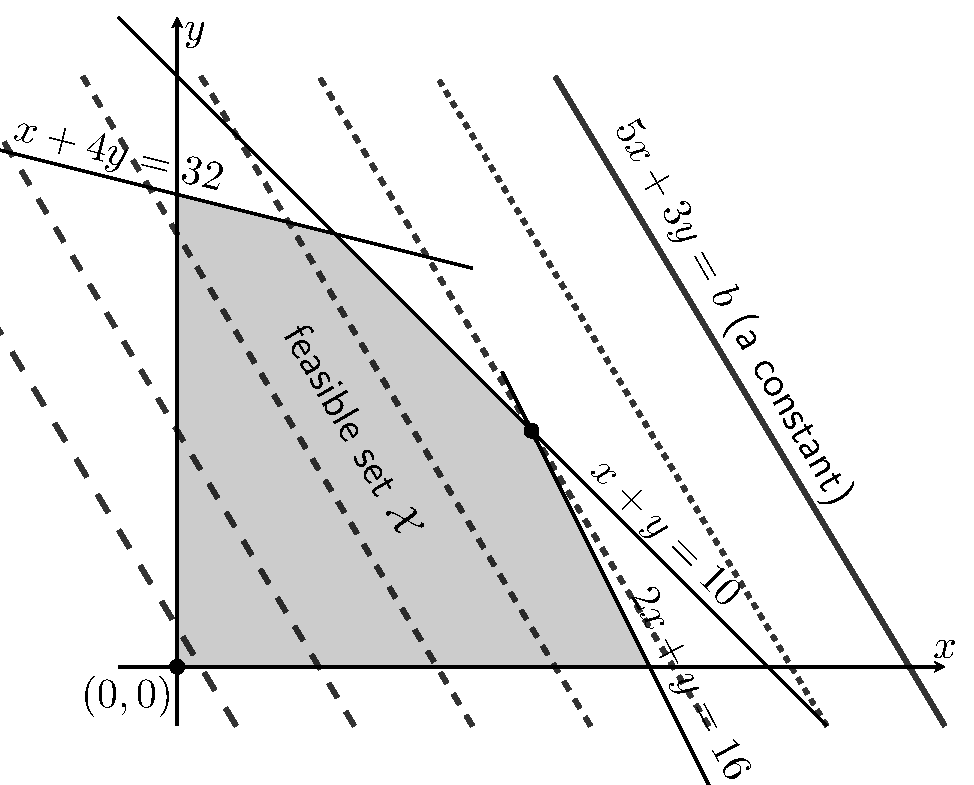
\includegraphics[width=8cm]{Chapters/08_ConvexOptimization/17_convexopt/latex/planting.pdf}}
    % 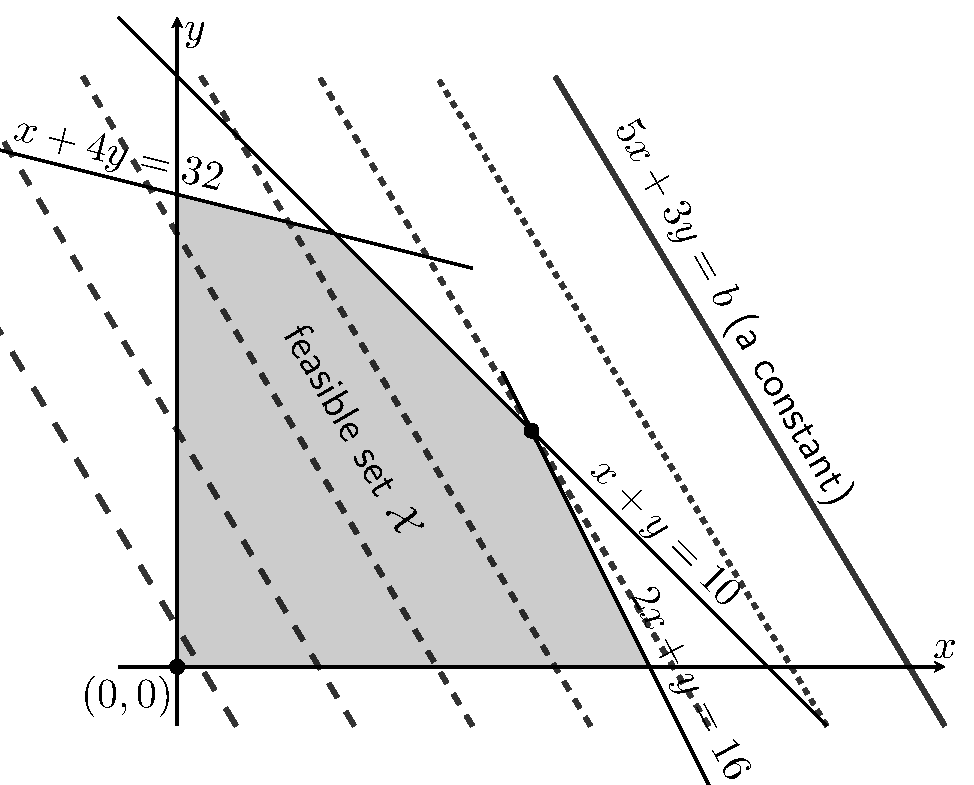
\includegraphics[width=8cm]{Chapters/08_ConvexOptimization/17_convexopt/latex/planting.pdf}ML
\end{figure}
% ******************************************************************************
 
Có thể nhận thấy nghiệm của bài toán chính là giao điểm của hai đường thẳng $x +
y = 10$ và $2x + y = 16$. Giải hệ phương trình này ta có $x^* = 6$ và $y^* = 4$.
Tức anh nông dân nên trồng 6 ha cà phê và 4 ha hồ tiêu. Lúc đó lợi nhuận thu được
là $5x^* + 3y^* = 42 $ triệu đồng và chỉ mất thời gian là 22 ngày.
Trong khi đó, nếu trồng toàn bộ hồ tiêu trong 32 ngày, tức 8 ha, anh chỉ thu được
24 triệu đồng.
 
Với các bài toán tối ưu có nhiều biến và ràng buộc hơn, sẽ rất khó để
minh hoạ và tìm nghiệm bằng cách này. Chúng ta cần có một công cụ hiệu quả hơn để tìm nghiệm bằng cách lập trình.

\subsection{Bài toán đóng thùng}
 
\textit{Bài toán}: Một công ty phải chuyển 400 $m^3$ cát tới địa điểm xây dựng ở
bên kia sông bằng
cách thuê một chiếc xà lan. Ngoài chi phí vận chuyển 100k cho một lượt đi về, công ty  phải thiết kế một thùng hình hộp chữ nhật không cần nắp đặt trên xà
lan để đựng cát. Chi phí sản xuất các mặt xung quanh
là 1 tr/$m^2$ và mặt đáy là 2 tr/$m^2$. Để tổng chi phí vận chuyển là nhỏ nhất, chiếc thùng cần được thiết kế như thế nào? Để đơn giản hóa bài toán, giả sử cát chỉ được
đổ ngang hoặc thấp hơn với phần trên của thành thùng, không đổ thành ngọn. Để đơn giản hơn nữa, giả sử thêm rằng xà lan có thể chở được thùng có kích thước vô hạn và khối lượng vô hạn (không được đổ trực tiếp cát lên mặt xà lan). 
 
 
\textit{\textbf{Phân tích}}

Giả sử chiếc thùng cần làm có chiều dài, chiều rộng, chiều cao lần lượt là $x,
y, z$ (m). Thể tích của thùng là $xyz$ ($m^3$). Có hai loại chi phí:
\begin{itemize}
    \item \textit{Chi phí thuê xà lan}: Số chuyến xà lan phải thuê\footnote{Ta
    hãy tạm giả sử rằng đây là một số tự nhiên, việc làm tròn này sẽ không thay
    đổi kết quả đáng kể vì chi phí vận chuyển một chuyến là nhỏ so với chi phí
    làm thùng} là $\frac{400}{xyz}$. Số tiền phải trả cho xà lan là
    $\displaystyle 0.1\frac{400}{xyz} = \frac{40}{xyz} = 40x^{-1}y^{-1}z^{-1}$
    (0.1 ở đây là 0.1 triệu đồng).
    \item \textit{Chi phí làm thùng}: Diện tích xung quanh của thùng là $2 (x +
    y)z $. Diện tích đáy là $xy$. Vậy tổng chi phí làm thùng là $2(x +y)z + 2xy
    = 2(xy + yz + zx)$.
\end{itemize}
 
Tổng toàn bộ chi phí là $f(x, y, z) = 40x^{-1}y^{-1}z^{-1} + 2(xy + yz + zx)$.
Điều kiện ràng buộc duy nhất là kích thước thùng phải dương. Vậy ta có
bài toán tối ưu sau.  

% \myrule

\textit{\textbf{Bài toán vận chuyển}}:
\begin{equation} 
\begin{aligned}
    (x, y) &= \arg\min_{x, y, z} 40x^{-1}y^{-1}z^{-1} + 2(xy + yz + zx) \\\ 
    \text{thoả mãn:}~ & x, y, z > 0
\end{aligned}
\end{equation} 
% \myrule
Bài toán này thuộc loại \textit{quy hoạch hình học} \textit{{geometric programming, GP)}}. Định nghĩa của GP
và cách dùng công cụ tối ưu sẽ được trình bày trong phần sau của chương.
 
\textit{Nhận thấy rằng bài toán này hoàn toàn có thể giải được bằng bất
đẳng thức Cauchy, nhưng chúng ta muốn một lời giải tổng quát cho bài toán để có thể lập trình được.}
 
(Lời giải:  
% \begin{equation*} 
    $f(x, y, z)= \frac{20}{xyz} + \frac{20}{xyz} + 2xy + 2yz + 2zx
    \geq 5\sqrt[5]{3200} $.
% \end{equation*} 
Dấu bằng xảy ra khi và chỉ khi $x = y = z = \sqrt[5]{10}$.) 
 
Khi có các ràng buộc về kích thước của thùng và trọng lượng mà xà lan tải được
thì bài toán trở nên phức tạp hơn, và bất đẳng thức Cauchy không phải lúc nào cũng làm việc hiệu quả. 

\index{bài toán tối ưu -- optimization problem}

Những bài toán trên đây đều là các bài toán tối ưu. Chính xác hơn, chúng đều
là các \textit{bài toán tối ưu lồi} ({convex optimization problems}). Trước hết, chúng ta cần hiểu các khái niệm cơ bản trong một bài toán tối ưu. 
 
 
\section{Nhắc lại bài toán tối ưu}
 
\subsection{Các khái niệm cơ bản}
Bài toán tối ưu ở dạng tổng quát:  
\begin{equation} 
\label{eqn:17_optprob1}
\begin{aligned}
\mathbf{x}^* &= \arg\min_{\mathbf{x}} f_0(\mathbf{x}) \\\ 
\text{thoả mãn:}~ & f_i(\mathbf{x}) \leq 0, ~~ i = 1, 2, \dots,m \\\ 
& h_j(\mathbf{x}) = 0, ~~ j = 1, 2, \dots, p 
\end{aligned}
\end{equation} 
 

 

 \begin{table}[t]
\centering
\caption{Bảng các thuật ngữ và ký hiệu trong bài toán tối ưu.}
\label{tab:17_terms}
\setlength{\tabcolsep}{0.5em}
{\small \def\arraystretch{1.5}
\begin{tabular}{|c|l|l|}
\hline
\multicolumn{1}{|c|}{\textbf{Ký hiệu}} & \multicolumn{1}{c|}{\textbf{Tiếng Anh}}
& \multicolumn{1}{c|}{\textbf{Tiếng Việt}} \\ \hline \hline 
 $\mathbf{x} \in \mathbb{R}^n$   & optimization variable                   & biến tối ưu                              \\ \hline
$f_0: \mathbb{R}^n \rightarrow \mathbb{R}$  & objective/loss/cost/function            & hàm mục tiêu                             \\ \hline
$f_i(\mathbf{x}) \leq 0 $  & inequality constraint                   & bất đẳng thức ràng buộc                  \\ \hline
 $f_i: \mathbb{R}^n \rightarrow \mathbb{R}$  & inequality constraint function          & hàm bất đẳng thức ràng buộc              \\ \hline
$h_j(\mathbf{x}) = 0 $   & equality constraint                     & đẳng thức ràng buộc                      \\ \hline
$h_j: \mathbb{R}^n \rightarrow \mathbb{R}$   & equality constraint function            & hàm đẳng thức ràng buộc                  \\ \hline
 $\mathcal{D} = \bigcap_{i=0}^m \text{\bf dom}f_i \cap \bigcap_{j=1}^p \text{\bf dom}h_j $  & domain                                  & tập xác định                             \\ \hline
\end{tabular}}
\end{table}

Phát biểu bằng lời: Tìm giá trị của biến $\mathbf{x}$ để tối thiểu hàm
$f_0(\mathbf{x})$ trong số những giá trị $\mathbf{x}$ thoả mãn các điệu kiện
ràng buộc. Ta có bảng khái niệm song ngữ và ký hiệu của bài toán tối ưu được trình bày  trong Bảng~\ref{tab:17_terms}. 

Ngoài ra:
\begin{itemize}
    \item Khi $m = p = 0$, bài toán \eqref{eqn:17_optprob1} được gọi là
    \textit{bài toán tối ưu không ràng buộc} ({unconstrained optimization
    problem}). 
     
    \item $\mathcal{D}$ là tập xác định, tức giao của tất cả các tập xác định
    của mọi hàm số xuất hiện trong bài toán. Tập hợp các điểm thoả mãn mọi điều
    kiện ràng buộc là một tập con của $\mathcal{D}$ được gọi là \textit{tập khả khi} (feasible set). Khi tập khả thi là một tập rỗng thì bài toán tối ưu \eqref{eqn:17_optprob1} \textit{bất khả thi} ({infeasible}). Một điểm nằm trong tập khả thi được gọi là \textit{điểm khả thi} (feasible point).
     
    \index{giá trị tối ưu -- optimal value}
    \item  \textit{Giá trị tối ưu} (optimal value) của bài toán tối ưu \eqref{eqn:17_optprob1} được định nghĩa là: 
    \begin{equation*} 
    p^* = \text{inf}\left\{f_0(\mathbf{x}) | f_i(\mathbf{x}) \leq 0, i = 1, \dots, m; h_j(\mathbf{x}) = 0, j = 1, \dots, p\right\} 
    \end{equation*} 
    $p^*$ có thể nhận các giá
    trị $\pm \infty$. Nếu bài toán là bất khả thi, ta coi $p^* = + \infty$, Nếu hàm mục tiêu
    không bị chặn dưới, ta coi
    $p^* = - \infty$.

\end{itemize}
 
 
% \subsection{Optimal và locally optimal points}
\subsection{Điểm tối ưu và tối ưu địa phương}

\index{die@điểm tối ưu -- optimal point}
\index{die@điểm tối ưu địa phương -- local optimal point}
Một điểm $\mathbf{x}^*$ được gọi là \textit{điểm tối ưu} ({optimal point})
, của bài toán
\eqref{eqn:17_optprob1} nếu $\mathbf{x}^*$ là một điểm khả thi và
$f_0(\mathbf{x}^*) = p^*$. Tập hợp tất cả các điểm tối ưu được gọi là
\textit{tập tối ưu} ({optimal set}). Nếu tập tối ưu khác rỗng,
ta nói bài toán \eqref{eqn:17_optprob1} \textit{giải được}
({solvable}). Ngược lại, nếu tập tối ưu rỗng, ta nói giá trị tối ưu không thể đạt được.
 
\textit{Ví dụ}: Xét hàm mục tiêu $f(x) = 1/x$ với ràng buộc $x > 0$. Giá trị tối ưu của bài toán này là $p^* = 0$ nhưng tập tối ưu là một tập rỗng
vì không có giá trị nào của $x$ để hàm mục tiêu đạt giá trị $p^*$. 
 
Với hàm một biến, một điểm là \textit{cực tiểu/tối ưu địa phương} của hàm số nếu tại đó hàm số
đạt giá trị nhỏ nhất trong một lân cận (và lân cận này thuộc tập xác định của
hàm số). Trong không gian một chiều, {lân cận} của một điểm được hiểu là
tập các điểm cách điểm đó một khoảng rất nhỏ. Trong không gian nhiều chiều, ta
gọi một điểm $\mathbf{x}$ là {tối ưu địa phương} nếu tồn tại một
giá trị $R > 0$ sao cho:
\begin{eqnarray} 
    \nonumber
    f_0(\mathbf{x}) = &\text{inf}\big\{f_0(\mathbf{z}) | f_i(\mathbf{z}) \leq 0, i = 1, \dots, m, \\
                 & h_j(\mathbf{z}) = 0, j = 1, \dots, p, \|\mathbf{z} - \mathbf{x}\|_2 \leq R\big\} 
\end{eqnarray} 
% Nếu một điểm khả thi $\mathbf{x}$ thoả mãn $f_i(\mathbf{x}) = 0$, ta
% nói rằng bất đẳng thức ràng buộc thứ $i$: $f_i(\mathbf{x}) = 0$ là
% \textit{active}. Nếu $f_i(\mathbf{x}) < 0$, ta nói rằng ràng buộc này là
% \textit{inactive} tại $\mathbf{x}$.
 
 
\subsection{Một vài lưu ý}
Bài toán trong định nghĩa \eqref{eqn:17_optprob1} là {tối thiểu hàm mục tiêu} với các ràng buộc nhỏ hơn
hoặc bằng không. Các bài toán yêu cầu {tối đa hàm mục tiêu} và điều kiện
ràng buộc ở dạng khác đều có thể đưa về được dạng này:
\begin{itemize}
    \item $\max f_0(\mathbf{x}) \Leftrightarrow\min -f_0(\mathbf{x}) $. 
     
    \item $f_i(\mathbf{x}) \leq g(\mathbf{x}) \Leftrightarrow\ f_i(\mathbf{x}) - g(\mathbf{x}) \leq 0$. 
     
    \item $f_i(\mathbf{x}) \geq 0 \Leftrightarrow\ -f_i(\mathbf{x}) \leq 0 $. 
     
    \item $a \leq f_i(\mathbf{x}) \leq b \Leftrightarrow\ f_i(\mathbf{x}) -b \leq 0$ và $a - f_i(\mathbf{x}) \leq 0$. 
     \index{biến lỏng lẻo -- slack variable}
    % \item $f_i(\mathbf{x}) \leq 0 \Leftrightarrow f_i(\mathbf{x}) + s_i = 0 $ và
    % $s_i \geq 0$. $s_i$ được gọi là \textit{slack variable}. Phép biến đổi đơn
    % giản này trong nhiều trường hợp lại tỏ ra hiệu quả vì bất đẳng thức $s_i
    % \geq 0$ thường dễ giải quyết hơn là $f_i(\mathbf{x}) \leq 0$.
    \item Trong nhiều trường hợp, ràng buộc $f_i(\bx) \leq 0$ được viết lại dưới dạng hai ràng buộc $f_i(\bx) + s_i = 0$ và $s_i \geq 0$. Biến được thêm vào $s_i$ được gọi là \textit{biến lỏng lẻo} (slack variable).   
    Ràng buộc không âm $s_i \geq 0$ nói chung dễ giải quyết hơn bất phương trình ràng buộc $f_i(\bx) \leq 0$.
\end{itemize}
 
\index{bài toán tối ưu lồi -- convex optimization problem}
\section{Bài toán tối ưu lồi}
 
% Trong toán tối ưu, chúng ta đặc biệt quan tâm tới những bài toán mà hàm mục tiêu
% là một hàm lồi, và tập khả thi cũng là một tập lồi.
 
\subsection{Định nghĩa}

\begin{mydef}{Bài toán tối ưu lồi}{def:convxoptprobs}

Một \textit{bài toán tối ưu lồi} ({convex optimization problem}) là một
bài toán tối ưu có dạng
\begin{equation} 
\label{eqn:17_cvxopt1}
\begin{aligned}
\mathbf{x}^* &= \arg\min_{\mathbf{x}} f_0(\mathbf{x}) \\\ 
\text{thoả mãn:}~ & f_i(\mathbf{x}) \leq 0, ~~ i = 1, 2, \dots, m \\\ 
% \nonumber
& h_j(\bx) = \mathbf{a}_j^T\mathbf{x} - b_j = 0, j = 1, \dots, 
\end{aligned}
\end{equation} 
trong đó $f_0, f_1, \dots, f_m$ là các hàm lồi. 
\end{mydef}
 
So với bài toán tối ưu \eqref{eqn:17_optprob1}, bài toán tối ưu lồi
\eqref{eqn:17_cvxopt1} có thêm ba điều kiện:

\begin{itemize}
    \item {Hàm mục tiêu} là một {hàm lồi}. 
     
    \item Các hàm bất đẳng thức ràng buộc $f_i$ là các hàm lồi. 
     
    \item Hàm đẳng thức ràng buộc $h_j$ là hàm {affine}.
\end{itemize}
Trong toán tối ưu, chúng ta đặc biệt quan tâm tới các bài toán tôi ưu lồi. 

Một vài nhận xét: 

\begin{itemize}
    \item Tập hợp các điểm thoả mãn $h_j(\mathbf{x}) = 0$ là một tập lồi vì nó
    có dạng siêu phẳng.
 
    \item Khi $f_i$ là một {hàm lồi}, tập hợp các điểm thoả mãn
    $f_i(\mathbf{x}) \leq 0 $ là tập dưới mức 0 của $f_i$ và là một tập
    lồi.
     
    \item Tập hợp các điểm thoả mãn mọi điều kiện ràng buộc là
    giao của các tập lồi, vì vậy nó là một tập lồi. 
\end{itemize}

\newnote{}{
Trong một bài toán tối ưu lồi, một hàm mục tiêu lồi được tối thiểu trên một tập
lồi.
}
 
 
\subsection{Cực trị địa phương của bài toán tối ưu lồi là cực trị toàn cục} 

Tính chất quan trọng nhất của bài toán tối ưu lồi chính là mọi điểm cực tiểu địa phương đều là cực tiểu toàn cục. Điều này có thể chứng minh bằng phản chứng. Gọi
$\mathbf{x}_0$ là một điểm cực tiểu địa phương:
\begin{equation*} 
f_0(\mathbf{x}_0) = \text{inf} \{f_0(\mathbf{x}) | \mathbf{x} \in
~\text{tập khả thi}, \|\mathbf{x} - \mathbf{x}_0\|_2 \leq R\} \end{equation*}
với $R > 0$ nào đó. Giả sử $\mathbf{x}_0$ không phải là một cực trị toàn cục, tức tồn tại một điểm khả thi $\mathbf{y}$
sao cho $f(\mathbf{y}) < f(\mathbf{x}_0)$ (hiển nhiên $\mathbf{y}$ không
nằm trong lân cận đang xét). Ta có thể tìm được $\theta \in [0, 1]$ sao
cho $\mathbf{z} = (1 - \theta)\mathbf{x}_0 + \theta\mathbf{y}$ nằm trong lân cận
của $\mathbf{x}_0$, tức $\|\mathbf{z} - \mathbf{x}_0\|_2 < R$. Việc này đạt được được
vì tập khả thi là một tập lồi. Hơn nữa, vì {hàm mục tiêu} $f_0$ là một
hàm lồi, ta có 
\begin{eqnarray} 
    f_0(\mathbf{z}) &=& f_0((1 - \theta)\mathbf{x}_0 + \theta \mathbf{y})  \\\ 
                    &\leq& (1 - \theta)f_0(\mathbf{x}_0) + \theta f_0(\mathbf{y})\\\ 
                    & < & (1 - \theta)f_0(\mathbf{x}_0) + \theta f_0(\mathbf{x}_0) 
                    = f_0(\mathbf{x}_0) 
\end{eqnarray} 
Điều này mâu thuẫn với giả thiết $\mathbf{x}_0$ là một điểm cực tiểu địa phương và $\bz$ nằm trong lân cận của $\bx_0$. Vậy giả thiết phản chứng là
sai, tức $\mathbf{x}_0$ chính là một điểm cực trị toàn cục. \dpcm 
 
Chứng minh bằng lời: Ggiả sử một điểm cực tiểu địa phương không phải là cực tiểu toàn cục. Vì hàm mục tiêu và tập khả thi đều lồi, ta luôn tìm được một điểm khác trong lân cận của điểm cực tiểu đó
sao cho giá trị của hàm mục tiêu tại điểm mới này nhỏ hơn giá trị của hàm mục
tiêu tại điểm cực tiểu. Sự mâu thuẫn này chỉ ra rằng với một bài toán tối ưu
lồi, điểm cực tiểu địa phương phải là điểm cực tiểu toàn cục. 
 
 

\subsection{Điều kiện tối ưu cho hàm mục tiêu khả vi}
 
Nếu hàm mục tiêu $f_0$ là khả vi, theo điều kiện bậc nhất, với mọi
$\mathbf{x}, \mathbf{y} \in \dom f_0$, ta có: 
\begin{equation} 
f_0(\mathbf{x}) \geq f_0(\mathbf{x}_0) + \nabla f_0(\mathbf{x}_0)^T (\mathbf{x} - \mathbf{x}_0)
\end{equation} 
Đặt $\mathcal{X}$ là tập khả thi. {Điều kiện cần và đủ} để một điểm $\mathbf{x}_0 \in \mathcal{X}$ là điểm tối ưu là: 
\begin{equation} 
\nabla f_0(\mathbf{x}_0)^T(\mathbf{x} - \mathbf{x}_0) \geq 0, ~\forall \mathbf{x} \in \mathcal{X} 
\end{equation} 
Phần chứng minh cho điều kiện này được bỏ qua, bạn đọc có thể tìm trong trang
139-140 của cuốn \textit{Convex Optimization}~\cite{boyd2004convex}.

\index{siêu phẳng hỗ trợ -- supporting hyperplane}

Điều này chỉ ra rằng nếu $\nabla f_0(\bx_0) = 0$ thì $\bx_0$ chính là một điểm
tối ưu của bài toán. Nếu $\nabla f_0(\bx_0) \neq 0$, nghiệm của bài toán sẽ
phải nằm trên biên của tập khả thi. Thật vậy, quan sát
Hình~\ref{fig:17_optimalitycondition}, điều kiện này nói rằng nếu $\mathbf{x}_0$
là một điểm tối ưu thì với mọi $\mathbf{x} \in \mathcal{X}$, vector đi từ
$\mathbf{x}_0$ tới $\mathbf{x}$ hợp với vector $-\nabla f_0 (\mathbf{x}_0)$ một
góc tù. Nói cách khác, nếu ta vẽ {mặt tiếp tuyến} của hàm mục tiêu tại
$\mathbf{x}_0$ thì mọi điểm {khả thi} nằm về một phía so với {mặt tiếp tuyến
này}. Điều này chỉ ra rằng $\bx_0$ phải nằm trên biên của tập khả thi
$\mathcal{X}$. Hơn nữa, tập khả thi nằm về phía làm cho hàm mục tiêu đạt giá
trị cao
hơn $f_0(\mathbf{x}_0)$. Mặt tiếp tuyến này được gọi là \textit{siêu phẳng hỗ trợ} ({supporting hyperplane}) của tập khả thi tại điểm $\mathbf{x}_0$.

% Nếu $\bx_0$ không nằm trên biên của feasible set, siêu mặt phẳng đi qua
% $\bx_0$ có vector pháp tuyến $-\nabla f_0(\bx_0)$ sẽ \textit{chia cắt} feasible
% set. Vì vậy, ta luôn có thể tìm được một điểm $\bx$ sao cho $\nabla
% f_0(\mathbf{x}_0)^T(\mathbf{x} - \mathbf{x}_0) < 0$.
% ******************************************************************************
\begin{figure}[t]    % caption on side     
    \floatbox[{\capbeside\thisfloatsetup{capbesideposition={right,top},capbesidewidth=6cm}}]{figure}[\FBwidth]
    {\caption{Biểu diễn hình học của điều kiện tối ưu cho hàm mục tiêu khả vi.
    Các đường nét đứt tương ứng với các đường đồng mức. Nét đứt càng ngắn ứng với giá trị càng cao.}
    \label{fig:17_optimalitycondition}}
    {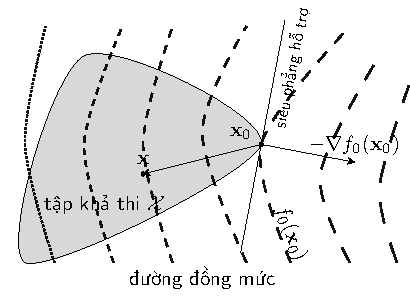
\includegraphics[width=8cm]{Chapters/08_ConvexOptimization/17_convexopt/latex/optimalitycondition_gray.pdf}}
\end{figure}
% ******************************************************************************
 
Một mặt phẳng đi qua một điểm trên biên của một tập hợp sao cho mọi điểm trong
tập hợp đó nằm về một phía (hoặc nằm trên) so với mặt phẳng đó được gọi là
một \textit{siêu phẳng hỗ trợ}. Tồn tại một siêu phẳng hỗ trợ tại mọi điểm trên biên của một tập lồi.
 
% Nếu tồn tại một điểm $\mathbf{x}_0$ trong \textit{feasible set} sao cho $\nabla
% f_0(\mathbf{x}_0) = 0$, đây chính là \textit{optimal point}. Điều này dễ hiểu vì
% đó chính là điểm làm cho gradient bằng 0, tức điểm cực tiểu của hàm mục tiêu.
% Nếu $\nabla f_0(\mathbf{x}_0) \neq 0$, vector $-\nabla f_0 (\mathbf{x}_0)$ chính
% là \textit{vector pháp tuyến} của \textit{supporting hyperplane} tại
% $\mathbf{x}_0$.
 
\index{CVXOPT} 
\subsection{Giới thiệu thư viện CVXOPT}
CVXOPT là một thư viện miễn phí trên Python đi kèm với cuốn sách \textit{Convex
Optimization}. Hướng dẫn cài đặt, tài liệu hướng dẫn, và các ví dụ mẫu của thư
viện này cũng có đầy đủ trên trang web CVXOPT (\url{http://cvxopt.org/}). Trong
phần còn lại của chương, chúng ta sẽ thảo luận ba bài toán cơ bản trong tối ưu lồi: quy hoạch tuyến tính, quy hoạch toàn phương và quy hoạch hình học. Chúng ta sẽ cùng lập trình để giải các ví dụ đã nêu ở phần đầu chương dựa trên thư viện CVXOPT này.
 
 
\section{Quy hoạch tuyến tính}
\index{quy hoạch tuyến tính -- linear programming}
Chúng ta cùng bắt đầu với lớp các bài toán \textit{quy hoạch tuyến tính} (linear programming, LP). Trong đó, hàm mục tiêu $f_0(\bx)$ và
các hàm bất đẳng thức ràng buộc $f_i(\bx), i = 1, \dots, m$ đều là hàm {affine}.
 
\subsection{Dạng tổng quát của quy hoạch tuyến tính}
% \myrule
\index{quy hoạch tuyến tính -- linear programming!dạng tổng quát -- general form}

\newnote{Dạng tổng quát của quy hoạch tuyến tính}{
\vspace{-.5cm}
\begin{eqnarray} 
\nonumber
\mathbf{x} &=& \arg\min_{\mathbf{x}} \mathbf{c}^T\mathbf{x} + d \\\ 
\label{eqn:17_generalLP}
\text{thoả mãn:}~ && \mathbf{Gx} \preceq \mathbf{h}\\\ 
\nonumber
&& \mathbf{Ax} = \mathbf{b} 
\end{eqnarray} 
Trong đó $\mathbf{G} \in \mathbb{R}^{m\times n}, \mathbf{h} \in \mathbb{R}^m$,
$\mathbf{A}\in \mathbb{R}^{p\times n}, \mathbf{b} \in\mathbb{R}^p$,
$\mathbf{c}, \mathbf{x} \in\mathbb{R}^n$ và $d\in \R$.
}
% \end{mydef}
Số vô hướng $d$ chỉ làm thay đổi giá trị của hàm mục tiêu mà không làm thay đổi
nghiệm của bài toán nên có thể được lược bỏ. Nhắc lại rằng ký hiệu $\preceq$
nghĩa là mỗi phần tử trong vector ở vế trái nhỏ hơn hoặc bằng phần tử tương ứng
trong vector ở vế phải. Các bất đẳng thức dạng
$\mathbf{g}_i\mathbf{x} \leq h_i$, với
$\mathbf{g}_i$ là những vector hàng, có thể viết gộp dưới dạng $\mathbf{Gx}
\preceq \mathbf{h}$ trong đó mỗi hàng của $\mathbf{G}$ ứng với một
$\mathbf{g}_i$, mỗi phần tử của $\mathbf{h}$ tương ứng với một $h_i$.
 
 
\subsection{Dạng tiêu chuẩn của quy hoạch tuyến tính}
Trong dạng tiêu chuẩn quy hoạch tuyến tính, bất phương trình ràng buộc
chỉ là điều kiện nghiệm có các thành phần không âm.

% \myrule
\index{quy hoạch tuyến tính -- linear programming!dạng tiêu chuẩn -- standard form}
% \textbf{A standard form LP:}  
% \begin{mydef}{Dạng tiêu chuẩn của Linear Programming}{def:standardLP}
\newnote{Dạng tiêu chuẩn của quy hoạch tuyến tính}{
\vspace{-.1cm}
\begin{equation} 
\label{eqn:17_standardLP}
\begin{aligned}
\mathbf{x} &= \arg\min_{\mathbf{x}} \mathbf{c}^T\mathbf{x} \\\ 
\text{thoả mãn:}~ & \mathbf{Ax} = \mathbf{b} \\\ 
& \mathbf{x} \succeq \mathbf{0} 
\end{aligned}
\end{equation}} 
% \end{mydef}
% \myrule
 
Dạng tổng quát \eqref{eqn:17_generalLP} có thể được đưa về dạng tiêu chuẩn
\eqref{eqn:17_standardLP} bằng cách đặt thêm biến lỏng lẻo $\mathbf{s}$:
\begin{equation} 
\label{eqn:17_21}
\begin{aligned}
\mathbf{x} &= \arg\min_{\mathbf{x}, \mathbf{s}} \mathbf{c}^T\mathbf{x} \\\ 
\text{thoả mãn:}~ & \mathbf{Ax} = \mathbf{b}\\\ 
& \mathbf{Gx} + \mathbf{s} = \mathbf{h} \\\ 
& \mathbf{s} \succeq \mathbf{0} 
\end{aligned}
\end{equation} 
Tiếp theo, nếu ta biểu diễn $\mathbf{x}$ dưới dạng hiệu của hai vector với thành
phần không âm: $\mathbf{x} = \mathbf{x}^+ - \mathbf{x}^-$, với
$\mathbf{x}^+, \mathbf{x}^- \succeq 0$. Ta có thể tiếp tục viết lại
\eqref{eqn:17_21} dưới dạng:
\begin{equation} 
\label{eqn:17_22}
\begin{aligned}
\mathbf{x} =& \arg\min_{\mathbf{x}^+,\mathbf{x}^-, \mathbf{s}} \mathbf{c}^T\mathbf{x}^+ - \mathbf{c}^T\mathbf{x}^- \\\ 
\text{thoả mãn:}~ & \mathbf{Ax}^+ - \mathbf{Ax}^- = \mathbf{b} \\\ 
& \mathbf{Gx}^+ - \mathbf{Gx}^- + \mathbf{s} = \mathbf{h} \\\ 
& \mathbf{x}^+ \succeq 0, \mathbf{x}^- \succeq 0, \mathbf{s} \succeq \mathbf{0} 
\end{aligned}
\end{equation} 
Tới đây, bạn đọc có thể thấy rằng \eqref{eqn:17_22} có dạng
\eqref{eqn:17_standardLP}.
 
 
\subsection{Minh hoạ bằng hình học của bài toán quy hoạch tuyến tính}
 
\begin{figure}[t]
    % caption on side     
    \floatbox[{\capbeside\thisfloatsetup{capbesideposition={right,top},
    capbesidewidth=6cm}}]{figure}[\FBwidth]
    {\caption{Biểu diễn hình học của quy hoạch tuyến tính}
    \label{fig:17_lp}}
    {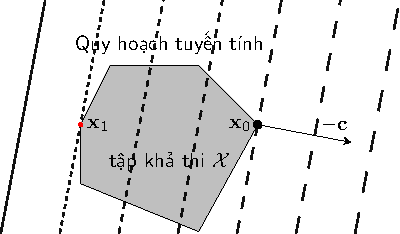
\includegraphics[width=7cm]{Chapters/08_ConvexOptimization/17_convexopt/latex/lp.pdf}}
\end{figure}
 
Các bài toán quy hoạch tuyến tính có thể được minh hoạ như Hình \ref{fig:17_lp} với tập khả thi có dạng đa diện lồi. Điểm
$\mathbf{x}_0$ là điểm cực tiểu toàn cục, điểm
$\mathbf{x}_1$ là điểm cực đại toàn cục. Nghiệm
của các bài toán quy hoạch tuyến tính, nếu tồn tại, là một điểm trên biên của của tập khả thi. 

% Tiếp theo, chúng ta sẽ dùng thư viện CVXOPT để giải các bài toán quy hoạch tuyến tính.
 
 
\subsection{Giải bài toán quy hoạch tuyến tính bằng CVXOPT}
 
Nhắc lại bài toán canh tác:
\begin{equation} 
\label{eqn:17_canhtac2}
\begin{aligned}
(x, y) =& \arg\max_{x, y} 5x + 3y \\\ 
\text{thoả mãn:}~ & x + y \leq 10 \\\ 
                    & 2x + y \leq 16  \\\ 
                    & x + 4y \leq 32 \\\ 
                    & x, y \geq 0 
\end{aligned}
\end{equation} 
Các điều kiện ràng buộc có thể viết lại dưới dạng $ \mathbf{Gx} \preceq
\mathbf{h}$, trong đó:
\begin{equation*} 
\mathbf{G} =  
\bmt
1 & 1 \\\ 
2 & 1 \\\ 
1 & 4 \\\ 
-1 & 0 \\\ 
0 & -1 
\emt
\mathbf{h} =  
\bmt
10\\\ 
16 \\\ 
32 \\\ 
0 \\\ 
0 
\emt
\end{equation*} 
 Khi sử dụng CVXOPT, chúng ta lập trình
như sau:
% \newpage 
\begin{lstlisting}[language=Python]
from cvxopt import matrix, solvers 
c = matrix([-5., -3.])  # since we need to maximize the objective funtion
G = matrix([[1., 2., 1., -1., 0.], [1., 1., 4., 0., -1.]]) 
h = matrix([10., 16., 32., 0., 0.]) 
 
solvers.options['show_progress'] = False 
sol = solvers.lp(c, G, h) 
 
print('Solution"') 
print(sol['x']) 
\end{lstlisting}
\kq 
\begin{lstlisting}[language=Python]
Solution: 
[ 6.00e+00] 
[ 4.00e+00] 
\end{lstlisting}
Nghiệm này chính là nghiệm mà chúng ta đã tìm được trong phần đầu của bài viết
dựa trên biểu diễn hình học. 
 
Một vài lưu ý: 

\begin{itemize}
    \item Hàm \pythoninline{solvers.lp} của \pythoninline{cvxopt} giải bài toán \eqref{eqn:17_21}. 
     
    \item Trong bài toán này, vì phải tìm giá trị lớn nhất nên hàm mục tiêu cần được đổi về dạng $-5x - 3y$. Vì vậy, ta cần khai báo \pythoninline{c = matrix([-5., -3.])}. 
     
    \item Hàm \pythoninline{matrix} nhận đầu vào là một \pythoninline{list} trong Python, \pythoninline{list} này thể hiện một vector cột. Nếu muốn biểu diễn một ma trận, đầu vào của \pythoninline{matrix} phải là một \pythoninline{list} của \pythoninline{list}, trong đó mỗi \pythoninline{list} bên trong thể hiện một vector cột. 
     
    \item Các hằng số trong bài toán phải ở dạng số thực. Nếu chúng là các số
    nguyên, ta cần thêm dấu chấm (\pythoninline{.}) để chuyển chúng thành số thực.
     
    \item Với đẳng thức ràng buộc $\mathbf{Ax} = \mathbf{b}$,
    \pythoninline{solvers.lp} lấy giá trị mặc định của \pythoninline{A} và
    \pythoninline{b} là \pythoninline{None}, tức nếu không khai báo thì không có đẳng thức ràng buộc nào.
    
\end{itemize}
Với các tuỳ chọn khác, bạn đọc có thể tìm trong tài liệu của CVXOPT(\url{https://goo.gl/q5CZmz}).
Việc giải Bài toán NXB bằng CVXOPT xin nhường lại cho bạn đọc.
 
\index{quy hoạch toàn phương -- quadratic programming}
\section{Quy hoạch toàn phương}
 
\subsection{Bài toán quy hoạch toàn phương}
Một dạng bài toán tối ưu lồi phổ biến khác là \textit{quy hoạch toàn phương} (quadratic
programming, QP). Khác biệt duy nhất của quy hoạch toàn phương so
với quy hoạch tuyến tính là hàm mục tiêu có \textit{dạng toàn phương} (\textit{quadratic form}).

% \begin{mydef}{Quadratic Programming}{def:quadraticprogramming}
\newnote{Quy hoạch toàn phương}{
\begin{equation} 
    \label{eqn:17_QP}
    \begin{aligned}
    \mathbf{x} &= \arg\min_{\mathbf{x}} \frac{1}{2} \mathbf{x}^T\mathbf{P}\mathbf{x} + \mathbf{q}^T\mathbf{x} + \mathbf{r} \\\ 
    \text{thoả mãn:}~ &\mathbf{Gx} \preceq \mathbf{h} \\\ 
    & \mathbf{Ax} = \mathbf{b} 
    \end{aligned}
\end{equation} 
Trong đó $\mathbf{P}$ là một ma trận vuông nửa xác định dương bậc $n$,
$\mathbf{G}\in \mathbb{R}^{m\times n}, \mathbf{A}\in\mathbb{R}^{p \times n}$. }

Điều kiện nửa xác định dương của $\bP$ nhằm đảm bảo hàm mục tiêu là lồi.
Trong quy hoạch toàn phương, một dạng toàn phương được tối thiểu trên một đa diện lồi (Xem
Hình~\ref{fig:17_qp}). Quy hoạch tuyến tính là một trường hợp đặc biệt của quy hoạch toàn phương với
$\mathbf{P} = \mathbf{0}$.
 

 
\subsection{Ví dụ}
\textit{Bài toán:} Một hòn đảo có dạng đa giác
lồi. Một con thuyền ở ngoài biển cần đi theo hướng nào để tới đảo nhanh
nhất, giả sử rằng tốc độ của sóng và gió bằng không. Đây chính là bài toán tìm khoảng cách từ
một điểm tới một đa diện. 
 
Bài toán tìm khoảng cách từ một điểm tới một đa diện: Cho
một đa diện là tập hợp các điểm thoả mãn $\mathbf{Ax} \preceq \mathbf{b}$ và
một điểm $\mathbf{u}$, tìm điểm $\mathbf{x}$ thuộc đa diện đó sao cho khoảng
cách Euclid giữa $\mathbf{x}$ và $\mathbf{u}$ là nhỏ nhất. Đây là một bài
toán quy hoạch toàn phương có dạng: 
\begin{eqnarray*} 
\mathbf{x} &=& \arg\min_{\mathbf{x}} \frac{1}{2}\|\mathbf{x} - \mathbf{u}\|_2^2 \\\ 
\text{thoả mãn:} &&\mathbf{Gx} \preceq \mathbf{h}
\end{eqnarray*} 
Hàm mục tiêu đạt giá trị nhỏ nhất bằng 0 nếu $\mathbf{u}$ nằm trong polyheron đó
và nghiệm chính là $\mathbf{x} = \mathbf{u}$. Khi $\mathbf{u}$ không nằm trong
polyhedron, ta viết:
\begin{equation*} 
\frac{1}{2} \|\mathbf{x} - \mathbf{u}\|_2^2 = \frac{1}{2} (\mathbf{x} - \mathbf{u})^T(\mathbf{x} - \mathbf{u}) = \frac{1}{2} \mathbf{x}^T\mathbf{x} - \mathbf{u}^T\mathbf{x} + \frac{1}{2} \mathbf{u}^T\mathbf{u} 
\end{equation*} 

Biểu thức này có dạng hàm mục tiêu như trong \eqref{eqn:17_QP} với $\mathbf{P = I}, \mathbf{q} = - \mathbf{u}, \mathbf{r} = \frac{1}{2} \mathbf{u}^T\mathbf{u}$, trong đó $\mathbf{I}$ là ma trận đơn vị. 

\begin{figure}[t]
    \floatbox[{\capbeside\thisfloatsetup{capbesideposition={right,top},capbesidewidth=6cm}}]{figure}[\FBwidth]
    {\caption{Biểu diễn hình học của quy hoạch toàn phương}
    \label{fig:17_qp}}
    {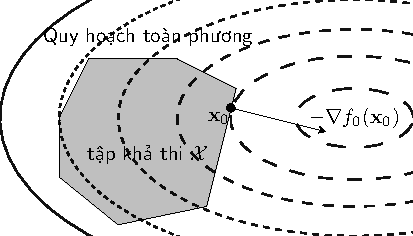
\includegraphics[width=8cm]{Chapters/08_ConvexOptimization/17_convexopt/latex/qp.pdf}}
\end{figure}
 
\subsection{Giải bài toán quy hoạch toàn phương bằng CVXOPT}
% ******************************************************************************
\begin{figure}[t]
    \floatbox[{\capbeside\thisfloatsetup{capbesideposition={right,top},capbesidewidth=5cm}}]{figure}[\FBwidth]
    {\caption{Ví dụ về khoảng cách giữa một điểm và một đa diện}
    \label{fig:17_qp_ex}}
    {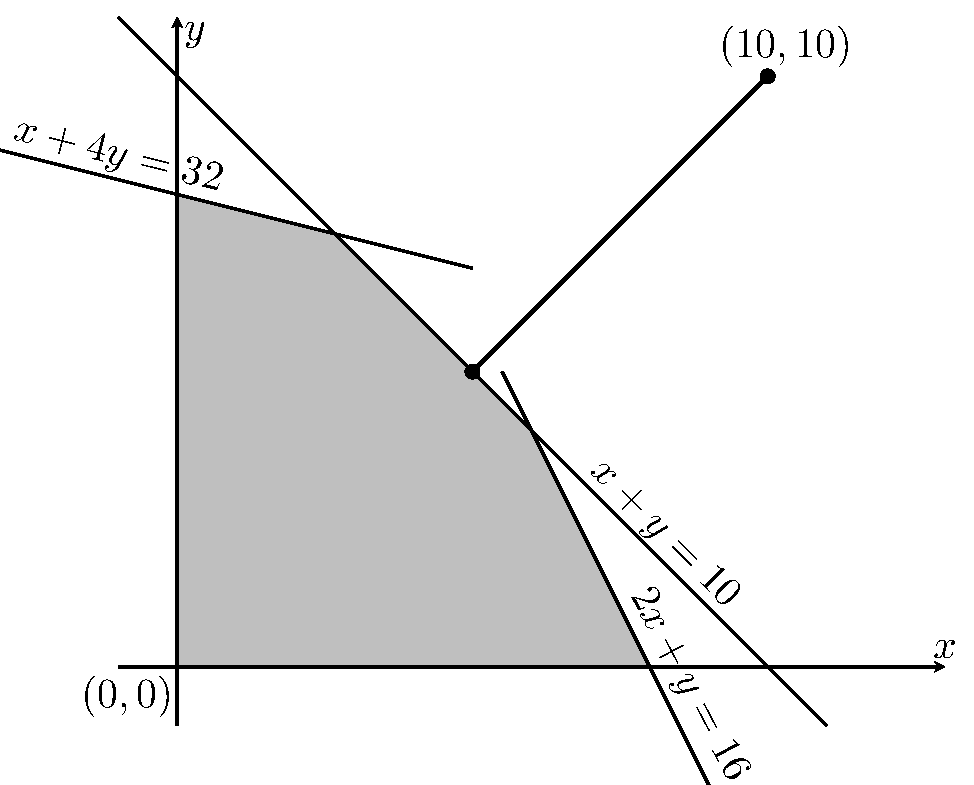
\includegraphics[width=8cm]{Chapters/08_ConvexOptimization/17_convexopt/latex/qp_ex.pdf}}
\end{figure}
% ******************************************************************************
Xét bài toán được cho trên Hình~\ref{fig:17_qp_ex}. Ta cần tìm khoảng cách từ
điểm có toạ độ $(10, 10)$ tới đa giác lồi màu xám. Khoảng cách từ một điểm
tới một tập hợp trong trường hợp này được định nghĩa là khoảng cách từ điểm đó
tới điểm gần nhất trong tập hợp. Bài toán này được viết dưới dạng quy hoạch toàn phương như sau:
\begin{eqnarray*} 
(x, y) &=& \arg\min_{x, y} (x - 10)^2 + (y - 10)^2 \\\ 
\text{thoả mãn:}~&& 
\bmt
1 & 1 \\\ 
2 & 1 \\\ 
1 & 4 \\\ 
-1 & 0 \\\ 
0 & -1 
\emt
\bmt
x \\\ 
y 
\emt
\preceq 
\bmt
10\\\ 
16 \\\ 
32 \\\ 
0 \\\ 
0 
\emt
\end{eqnarray*} 
Tập khả thi của bài toán được lấy từ Bài toán canh tác và
$\mathbf{u} = [10, 10]^T$. Bài toán này có thể được giải bằng CVXOPT như sau:
\newpage
\begin{lstlisting}[language=Python]
from cvxopt import matrix, solvers 
P = matrix([[1., 0.], [0., 1.]]) 
q = matrix([-10., -10.]) 
G = matrix([[1., 2., 1., -1., 0.], [1., 1., 4., 0., -1.]]) 
h = matrix([10., 16., 32., 0., 0]) 
 
solvers.options['show_progress'] = False 
sol = solvers.qp(P, q, G, h) 
 
print('Solution:') 
print(sol['x']) 
\end{lstlisting}
% \newpage 
\kq 
\begin{lstlisting}[language=Python]
Solution: 
[ 5.00e+00] 
[ 5.00e+00] 
\end{lstlisting}
Như vậy, nghiệm của bài toán tối ưu này là điểm có toạ độ $(5, 5)$ .
 
\section{Quy hoạch hình học}
\index{quy hoạch hình học -- geometric programming}
Trong mục này, chúng ta cùng thảo luận một nhóm các bài toán {không lồi}, nhưng có thể được biến đổi về
dạng {lồi}. Trước hết, ta
làm quen với hai khái niệm đơn thức và {đa thức}.
 
\subsection{Đơn thức và đa thức}
\index{don@đơn thức -- monomial} 
\index{da@đa thức -- posynomial} 
Một hàm số $f: \mathbb{R}^n \rightarrow \mathbb{R}$ với tập xác định $\text{dom}f = \mathbf{R}_{++}^n$ (tất cả các phần tử đều dương) có dạng:
\begin{equation} 
\label{eqn:17_monomials}
f(\mathbf{x}) = c x_1^{a_1} x_2^{a_2} \dots x_n^{a_n}
\end{equation} 
trong đó $c > 0$ và $a_i \in \mathbb{R}$, được gọi là một \textit{đơn thức} (monomial) (trong chương trình phổ
thông, đơn thức được định nghĩa với $c$ bất kỳ và $a_i$ là các số tự
nhiên).
 
Tổng của các đơn thức:
\begin{equation} 
\label{eqn:17_posy}
f(\mathbf{x}) = \sum_{k=1}^K c_k x_1^{a_{1k}}x_2^{a_{2k}}\dots x_n^{a_{nk}}
\end{equation} 
trong đó $c_k > 0$, được gọi là \textit{đa thức} (posynomial).
 
 
\subsection{Quy hoạch hình học}
% \begin{mydef}{Geometric Programming}{def:geometricprogramming}
     
\newnote{Quy hoạch hình học}{
\begin{equation} 
\label{eqn:17_25}
\begin{aligned}
\mathbf{x}   &= \arg\min_{\mathbf{x}} f_0(\mathbf{x}) \\\ 
\text{thoả mãn:}~ & f_i(x) \leq 1,  ~~ i = 1, 2, \dots, m\\\ 
                    & h_j(x) = 1, ~~ j = 1, 2, \dots, p 
\end{aligned}
\end{equation} 
trong đó $f_0, f_1, \dots, f_m$ là các đa thức và $h_1, \dots, h_p$
là các đơn thức.
}

Điều kiện $\mathbf{x} \succ 0$ đã được ẩn đi. 
 % \end{mydef} 
 
Chú ý rằng nếu $f$ là một đa thức, $h$ là một đơn thức thì $f/h$ là một đa thức. 
% \newpage

Ví dụ, bài toán tối ưu 
\begin{eqnarray} 
\nonumber
    (x, y, z)    &=& \arg\min_{x, y, z} x/y                          \\\ 
\text{thoả mãn:}~ && 1 \leq x \leq 2 \\\ 
\nonumber
 && x^3 + 2y/z \leq \sqrt{y} \\\ 
\nonumber
 && x/y = z 
\end{eqnarray} 
có thể được viết lại dưới dạng quy hoạch hình học:
\begin{eqnarray} 
\nonumber
    (x, y, z)    &=& \arg\min_{x, y, z} xy ^{-1}                        \\\ 
\text{thoả mãn:}~ && x^{-1} \leq 1 \\\ 
\nonumber
&& (1/2)x \leq 1 \\\ 
\nonumber
&& x^3y^{-1/2} + 2y^{1/2}z^{-1} \leq 1 \\\ 
\nonumber
&& xy^{-1}z^{-1} = 1 
\end{eqnarray} 
Bài toán này không là một bài toán tối ưu lồi vì cả hàm mục tiêu và điều kiện ràng buộc đều không lồi. 
 
 
\subsection{Biến đổi quy hoạch hình học về dạng bài toán tối ưu lồi}
Quy hoạch hình học có thể được biến đổi về dạng lồi bằng cách sau đây. Đặt $y_i = \log(x_i)$,
tức $x_i = \exp({y_i})$. Nếu $f$ là một đơn thức của
$\mathbf{x}$ thì:
\begin{equation*} 
f(\mathbf{x}) = c(\exp({y_1}))^{a_1} \dots (\exp({y_n}))^{a_n} =
c\exp\left(\sum_{i=1}^n a_iy_i\right) = \exp({\mathbf{a}^T\mathbf{y} + b}) 
\end{equation*} 
với $b = \log(c)$. Lúc này, hàm số $g(y) = \exp({\mathbf{a}^T\mathbf{y} + b})$ là một hàm lồi theo $\mathbf{y}$. (Bạn đọc có thể chứng minh theo định nghĩa rằng hợp của hai hàm lồi là một hàm lồi. Trong trường hợp này, hàm $\exp$ và hàm {affine} đều là các hàm lồi.) 
 
Tương tự, đa thức trong đẳng thức~\eqref{eqn:17_posy} có thể
được viết dưới dạng:
\begin{equation*} 
f(\mathbf{x}) = \sum_{k = 1}^K \exp(\mathbf{a}_k^T\mathbf{y} + b_k) 
\end{equation*} 
trong đó $\mathbf{a}_k = [a_{1k}, \dots, a_{nk}]^T, b_k = \log(c_k)$ và $y_i =
\log(x_)$. Lúc này, đa thức đã được viết dưới dạng tổng của các hàm
$\exp$ của các hàm {affine}, và vì vậy là một hàm lồi theo $\by$. Lưu ý rằng tổng của các hàm lồi là một hàm lồi.
% \newpage 

Bài toán quy hoạch hình học \eqref{eqn:17_25} được viết lại dưới dạng:  
\begin{equation} 
\label{eqn:17_26}
\begin{aligned}
    \mathbf{y} &= \arg\min_{\mathbf{y}} \sum_{k=1}^{K_0}
    \exp(\mathbf{a}_{0k}^T\mathbf{y} + b_{0k})                      \\\ 
\text{thoả mãn:}~ & \sum_{k=1}^{K_i} \exp(\mathbf{a}_{ik}^T\mathbf{y} + b_{ik}) \leq 1, ~~i = 1, \dots, m\\\ 
& \exp(\mathbf{g}_j^T\mathbf{y} + h_j) = 1, ~ j= 1, \dots, p 
    \end{aligned}
\end{equation} 
với $\mathbf{a}_{ik} \in \mathbb{R}^n,~\forall i = 1, \dots, p$ và $\mathbf{g}_j
\in
\mathbb{R}^n,~\forall j = 1, \dots, p$. 
 
Với chú ý rằng hàm số $\log \left(\sum_{i=1}^m
\exp(g_i(\mathbf{\bz}))\right)$ là môt hàm \textit{lồi} theo $\bz$ nếu $g_i$ là
các hàm {lồi} (xin bỏ qua phần chứng minh), ta có thể viết lại bài
toán \eqref{eqn:17_26} dưới dạng một bài toán tối ưu lồi bằng cách lấy $\log$ của các hàm như sau.

% \index{Geometric programming!convex form}
\textbf{\textit{{Quy hoạch hình học dưới dạng bài toán tối ưu lồi}}}
\begin{equation} 
 \label{eqn:17_27}
 \begin{aligned}
    \text{min}_{\mathbf{y}} \tilde{f}_0(\mathbf{y}) &= \log\left(\sum_{k=1}^{K_0} \exp(\mathbf{a}_{0k}^T \mathbf{y} + b_{i0})\right) \\
\text{thoả mãn:}~ \tilde{f}_i(\mathbf{y}) &= \log \left(\sum_{k=1}^{K_i} \exp(\mathbf{a}_{ik}^T \mathbf{y} + b_{ik})\right) \leq 0, ~~ i = 1, \dots, m \\ 
\tilde{h}_j(\mathbf{y}) &= \mathbf{g}_j^T\mathbf{y} + h_j = 0,~~ j = 1, \dots, p
 \end{aligned}
\end{equation} 
Lúc này, ta có thể nói rằng quy hoạch hình học tương đương với một bài toán tối ưu lồi vì hàm
mục tiêu và các hàm bất phương trình ràng buộc trong \eqref{eqn:17_27} đều là hàm
lồi, đồng thời ràng buộc phương trình cuối cùng có dạng {affine}. 
 
 
\subsection{Giải quy hoạch hình học bằng CVXOPT}
Quay lại ví dụ về Bài toán đóng thùng {không ràng buộc} và hàm mục
tiêu $f(x, y, z) = 40x^{-1}y^{-1}z^{-1} + 2xy + 2yz + 2zx$ là một đa thức. 
Vậy đây cũng là một bài toán quy hoạch hình học. 
 
Nghiệm của bài toán có thể được tìm bằng CVXOPT như sau:
\begin{lstlisting}[language=Python]
from cvxopt import matrix, solvers 
from math import log, exp# gp 
from numpy import array 
import numpy as np 
 
K = [4] # number of monomials
F = matrix([[-1., 1., 1., 0.], 
            [-1., 1., 0., 1.], 
            [-1., 0., 1., 1.]]) 
g = matrix([log(40.), log(2.), log(2.), log(2.)]) 
solvers.options['show_progress'] = False 
sol = solvers.gp(K, F, g) 
 
print('Solution:') 
print(np.exp(np.array(sol['x']))) 
 
print('\nchecking sol^5') 
print(np.exp(np.array(sol['x']))**5) 
\end{lstlisting}
% \newpage 
\kq 
\begin{lstlisting}[language=Python]
Solution: 
[[ 1.58489319] 
 [ 1.58489319] 
 [ 1.58489319]] 
 
checking sol^5 
[[ 9.9999998] 
 [ 9.9999998] 
 [ 9.9999998]] 
\end{lstlisting}
 
Nghiệm thu được chính là $x = y = z = \sqrt[5]{10}$. Bạn đọc nên
đọc thêm chỉ dẫn của hàm \pythoninline{solvers.gp} (\url{https://goo.gl/5FEBtn})
để hiểu cách thiết lập và giải bài toán quy hoạch hình học.
 
 
\section{Tóm tắt}
\begin{itemize}
    \item Các bài toán tối ưu xuất hiện rất nhiều trong thực tế, trong đó tối ưu
    lồi đóng một vai trò quan trọng. Trong bài toán tối ưu lồi, nếu tìm được cực
    trị địa phương thì đó chính là cực trị toàn cục.
     
    \item Có những bài toán tối ưu không được viết dưới dạng lồi nhưng có thể
    biến đổi về dạng lồi, ví dụ như bài toán quy hoạch hình học.
     
    \item Quy hoạch tuyến tính và quy hoạch hình học đóng một vai trò quan
    trọng trong toán tối ưu, được sử dụng nhiều trong các thuật toán machine
    learning.
     
    \item Thư viện CVXOPT được dùng để giải nhiều bài toán tối ưu lồi, rất dễ
    sử dụng, phù hợp với mục đích học tập và nghiên cứu. 
 
\end{itemize}
 
% \section{Tài liệu tham khảo}
% [1] \href{http://stanford.edu/~boyd/cvxbook/}{Convex Optimization} – Boyd and Vandenberghe, Cambridge University Press, 2004. 
 
% [2] \href{http://cvxopt.org/}{CVXOPT}. 
